\section{Pure approach}
\subsection{General}
\subsubsection{Performance}
Ground truth vs. pure, commission, image quantity 

The workers motivate their votes as follows: 
\begin{itemize}
	\item Higher value of information 
	\item Professionalism 
	\item Hidden information are given (e.g. size of the cleats, size of the smartphone storage) 
	\item The description is clear, short and to the point 
	\item Authenticity of the article 
	\item Grammatical issues 
\end{itemize}

\subsection{Title}
The length of the title (Figure \ref{crowdsourcing_title_length}) increases if the task contains all available pictures of the item. This setup produced an average title length of 64 characters. The other experiments have an average of 50 for the standard design and 48 for a promised commission. The median value shows almost the same ranking except the additional reward in form of a commission generates more characters than the standard configuration. The item without a brand was described by a title with 37 characters. The length doesn't say anything about the quality of the title, but it indicates the influence of the different task settings. The usage of natural language processing tools could help to get more information about the quality, but this would be outside the scope of the thesis.
\begin{figure}
\centering
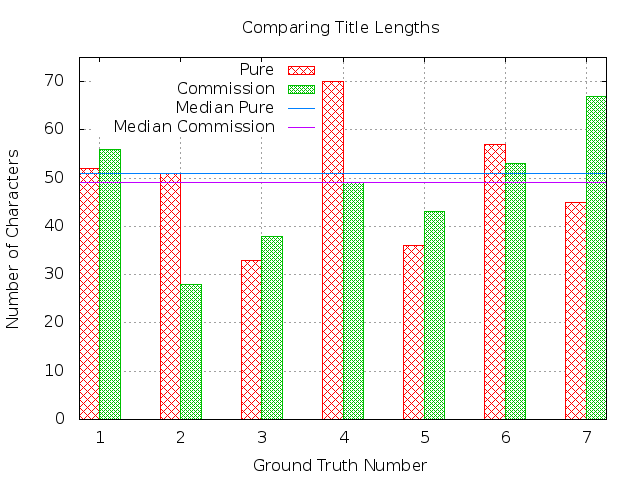
\includegraphics[scale=0.55]{images/plots/crowdsourcing/plot_title_length.png}
\caption{Evaluation of Title Lengths}
\label{crowdsourcing_title_length}
\end{figure} 

After the creation of the titles, the workers had to select the final one for each item. They justify their selections as follows:
\begin{itemize}
	\item Amount of details 
	\item Attracts more attention 
	\item Research on eBay produces better results for the title 
	\item Experiences with online auctions 
	\item Wrong information 
	\item Too long 
\end{itemize}

\subsection{Description}
The same measurements as for the title were done for the description (Figure \ref{crowdsourcing_desc_length}). The general task design achieved the highest average length (467 chars), but it contains an outlier with 1706 characters for the ground truth item number 5. The worker copied an item description from the website of the producer. More images doesn't conclude to a longer description, because the average length of these titles is 281. An extra reward leads to 455 characters, but has the highest median of 572. The numeric parameter is more robust to outliers. The other setups follow by 307 (Commission) and 238 (Pure). The non-branded item realise a length of 240 characters which is equal to the median of the branded items. Therefore, the workers are able to write descriptions of equal length regardless of which item type (branded/non-branded) was presented to them.
\begin{figure}
\centering
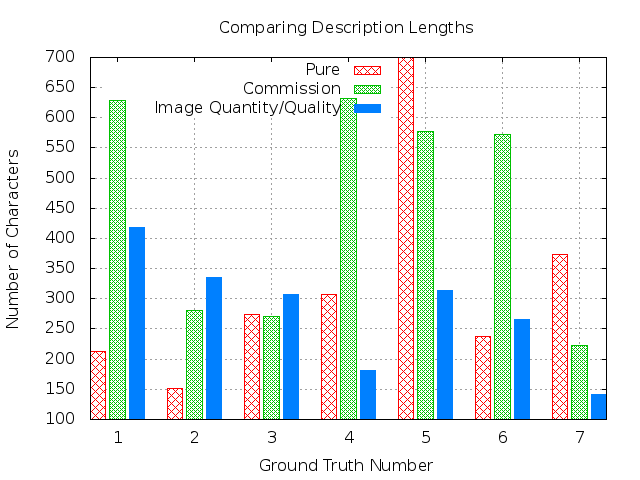
\includegraphics[scale=0.55]{images/plots/crowdsourcing/plot_description_length.png}
\caption{Evaluation of Description Lengths}
\label{crowdsourcing_desc_length}
\end{figure}

\subsection{Category}

\subsection{Price Estimation}
To evaluate the accuracy of the price estimations (Figure \ref{crowdsourcing_price_pred}), the root mean squared error (RMSE) was used. It is frequently used to measure the quality of predictions. The true values are the end prices from the ground truth. If the workers have the actual market price of the item at one's disposal then they predict the price best with an average RMSE of 51.46 USD. The experiment with the commission ranked just behind with 58.55 USD, the others appear with 81.75 (Pure) and 89.89 (Image quantity/quality) at the end of the ranking. The tested item without a brand has a RMSE of 278.62 USD which indicates the challenge of the price prediction for generic things.
Under/Over estimations
\begin{figure}
\centering
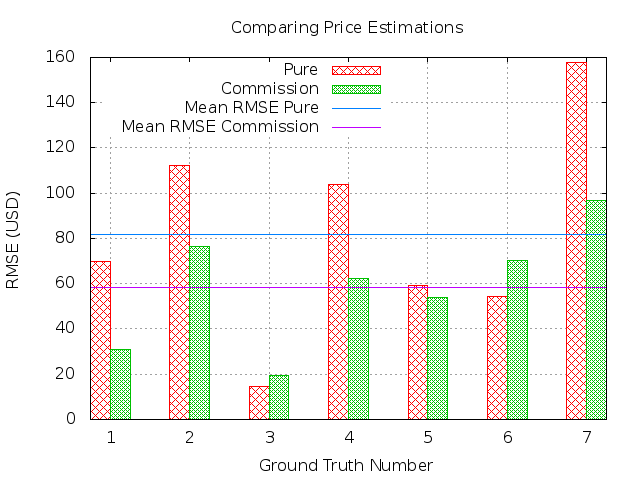
\includegraphics[scale=0.55]{images/plots/crowdsourcing/plot_price_rmse.png}
\caption{Price Prediction Quality}
\label{crowdsourcing_price_pred}
\end{figure}

\subsection{Variations}
\subsubsection{Commission }
The ground truth items 1 and 3 received a majority of the votes from the crowd. The commissions were paid manually using the web interface of the Amazon Mechanical Turk web service. The value of the bonus has to be shortened to two digits after the point and rounded up to \$0.01, because of some restrictions of MTurk. The bonus aggregates to \$1.48 for both auctions. The worker received also an additional message: \\
''Dear worker, \\

You receive a commission (0.25\% of the end price) as bonus payment for your work. The end price of the eBay online auction was \$27.''
\begin{table}[h!]
	\begin{center}
	\begin{tabular}{| p{1cm} | p{1.5cm} | p{3cm} | p{1.5cm} | p{1.5cm} | p{3.5cm} |}
		\hline
		Ground truth number & End price (USD) & Task & Percentage & Bonus (USD) & Worker ID \\
		\hline
		1 & 4.99 & Title (Finding) & 0.25\% & 0.01 & A3HE1W5T6QO03X \\
		\hline
		1 & 4.99 & Title (Voting) & 0.1\% & 0.01 & A3N7O1NOBGX6U7 \\
		\hline
		1 & 4.99 & Title (Voting) & 0.1\% & 0.01 & A1DK26QAO4OOMQ \\
		\hline
		1 & 4.99 & Description (Improving) & 1\% & 0.05 & A2Y9ZNZ0F24GHB \\
		\hline
		1 & 4.99 & Description (Voting) & 0.05\% & 0.01 & A2FF8HA1OWKS83 \\
		\hline
		1 & 4.99 & Description (Voting) & 0.05\% & 0.01 & AJAOE1PSNKGUE \\
		\hline
		1 & 4.99 & Category & 0.25\% & 0.01 & A2ZT4MTMEVSLB9 \\
		\hline
		1 & 4.99 & Category & 0.25\% & 0.01 & A220ED0LJITW5I \\
		\hline
		1 & 4.99 & Category & 0.25\% & 0.01 & A2V8WJXA0USMZ \\
		\hline
		1 & 4.99 & Price & 0.5\% & 0.02 & A3L99RGPK6FZGH \\
		\hline
		3 & 27 & Title (Finding) & 0.25\% & 0.06 & A23BCMQN9ZU97B \\
		\hline
		3 & 27 & Title (Voting) & 0.1\% & 0.02 & A3N7O1NOBGX6U7 \\
		\hline
		3 & 27 & Title (Voting) & 0.1\% & 0.02 & A3I4BYP4DUC475 \\
		\hline
		3 & 27 & Description (Improving) & 1\% & 0.27 & A1IA4CST74I1Q8 \\
		\hline
		3 & 27 & Description (Voting) & 0.05\% & 0.01 & A3K77RSYXLLUQL \\
		\hline
		3 & 27 & Description (Voting) & 0.05\% & 0.01 & A25F7BNXEN8I5X \\
		\hline
		3 & 27 & Category & 0.25\% & 0.06 & A2ZT4MTMEVSLB9 \\
		\hline
		3 & 27 & Category & 0.25\% & 0.06 & A220ED0LJITW5I \\
		\hline
		3 & 27 & Category & 0.25\% & 0.06 & A2V8WJXA0USMZ \\
		\hline
		3 & 27 & Price & 0.5\% & 0.13 & A3L99RGPK6FZGH \\
		\hline
	\end{tabular}
	\end{center}
	\caption{}
\end{table}



 

\section{Hybrid approach}
The Random Forest approach shows the best performance over all three item categories independent of classification or regression (Figure). The accuracy of the classifier depends also on the item category. The RFC assign every third input to the right Sony Playstation price class. The plot of the mean absolute error (MAE, Figure) assured the strength of the classifier and visualise how far away the predictions are in average. kNN has an error of about four classes for the iPhone category, one class has a range of 25 USD. The comparison between the human-based and the machine-based prediction indicates that the crowd can't be as accurate as a machine. The lowest RMSE of the ground truth item number 2 (Apple iPhone) is \$76.32. Two machine learning algorithms have a smaller error (Figure). 
The normalised confusion matrix (Figure) of the iPhone classifiers illustrates the distribution of the assignments. The origin is located at the left top position, the x-axis represents the truth-values and the y-axis the values assigned by the classifier. The values were normalised per row. A perfect classifier would produce a diagonal which contains only ones. 
The scatter plot (Figure) is another way to visualise the relations between the truth and predicted values. The criteria of a perfect classifier are the same as for the confusion matrix. 
The same plots for the other categories and the exact accuracies/RMSEs/MAEs are enumerated in the appendix section (Reference).
\begin{figure}
\centering
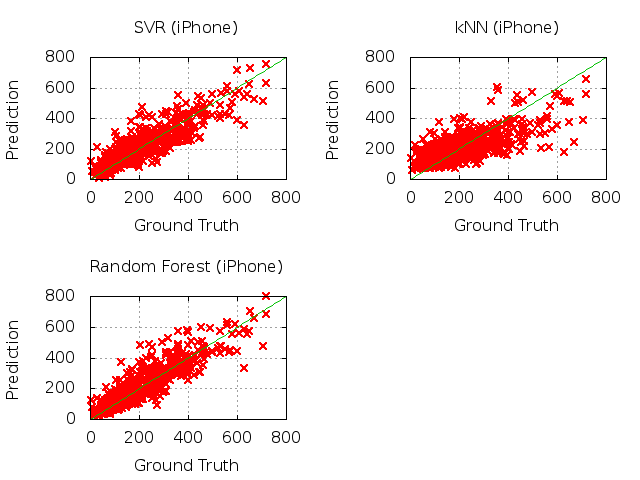
\includegraphics[scale=0.55]{images/plots/machine_learning/iphone/true_pred_iphone.png}
\caption{Scatter plot truth vs. prediction (iPhone)}
\label{truth_predict_iphone}
\end{figure}
\begin{figure}
\centering
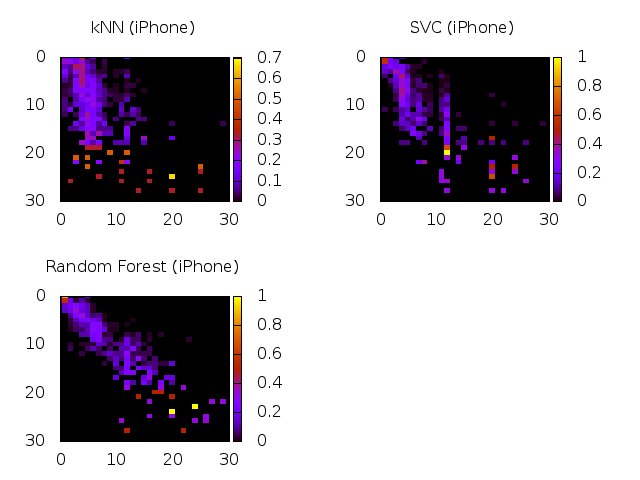
\includegraphics[scale=0.55]{images/plots/machine_learning/iphone/conf_mat_iphone.png}
\caption{Time/Error Function}
\label{crowdsourcing_desc_length}
\end{figure}

\begin{figure}
\centering
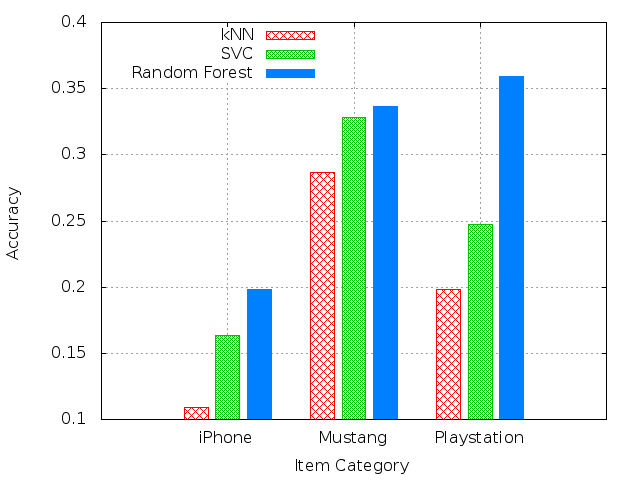
\includegraphics[scale=0.55]{images/plots/machine_learning/plot_price_classification_acc.png}
\caption{Time/Error Function}
\label{crowdsourcing_desc_length}
\end{figure}
\begin{figure}
\centering
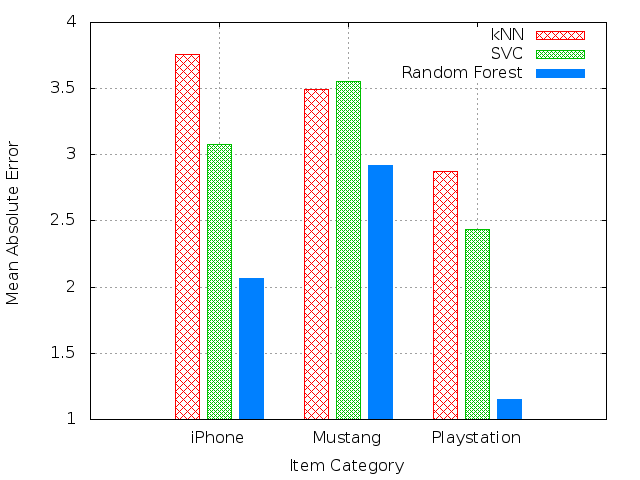
\includegraphics[scale=0.55]{images/plots/machine_learning/plot_price_classification_mae.png}
\caption{Time/Error Function}
\label{crowdsourcing_desc_length}
\end{figure}

\begin{figure}
\centering
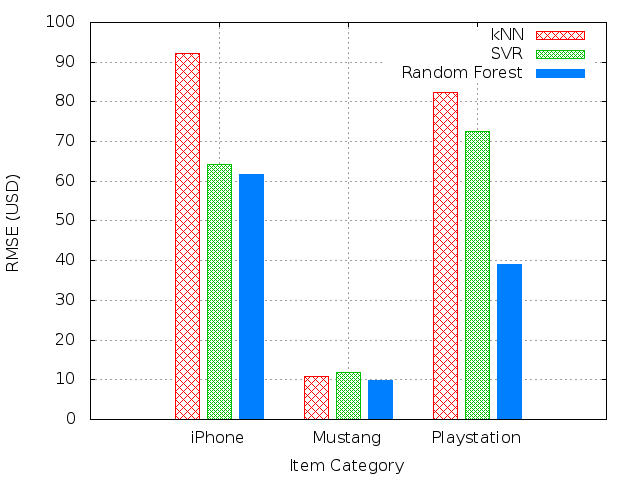
\includegraphics[scale=0.55]{images/plots/machine_learning/plot_price_regression_rmse.png}
\caption{Time/Error Function}
\label{crowdsourcing_desc_length}
\end{figure}




\begin{figure}
\centering
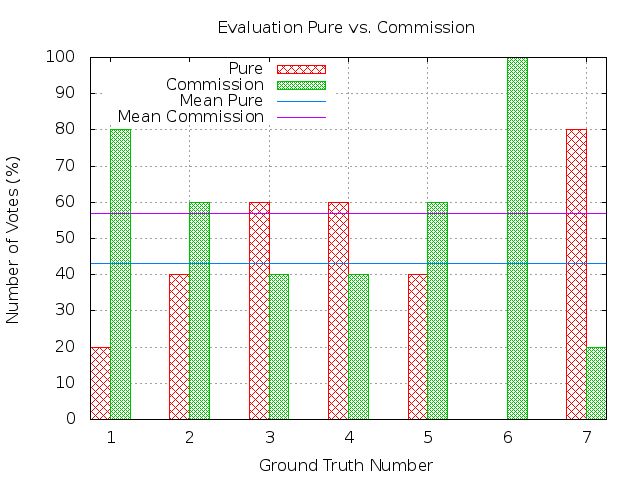
\includegraphics[scale=0.55]{images/plots/crowdsourcing/plot_evaluation_pure_vs_commission.png}
\caption{Evaluation of Pure vs. Commission}
\label{crowdsourcing_desc_length}
\end{figure}
\begin{figure}
\centering
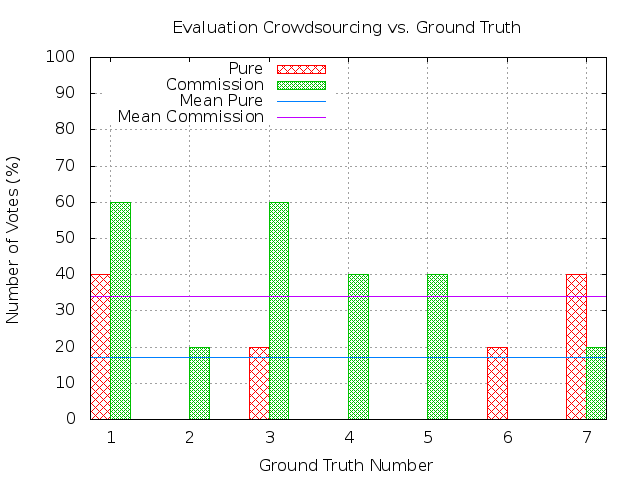
\includegraphics[scale=0.55]{images/plots/crowdsourcing/plot_evaluation_ground_vs_crowd.png}
\caption{Evaluation of Ground Truth vs. Crowdsourcing}
\label{crowdsourcing_desc_length}
\end{figure}


